\section{Distribución de los VO's en el mundo}

%\subsection{IVOA}

\begin{frame}
\frametitle{Distribución de los VO's en el mundo}

Desde el año 2002, proyectos de VO's comenzaron a integrar la International
Virtual Observatroy Alliance bajo el Guidelines for Participation
\footnote{\url{http://www.ivoa.net/documents/latest/IVOAParticipation.html}}.
\newline
\newline
Estos fueron fundados bajo programas privados y gubernamentales nacionales e
internacionales en colaboración con centro de estudios científicos,
universidades y otros. Quienes integran este proyecto, comparten conocimientos
entre ellos y la comunidad de modo estandarizado. Son ellos mismos quienes
desarrollan estos estándares para el intercambio de información e
interoperabilidad.

\end{frame}

\newpage

\begin{frame}
\frametitle{Distribución actual por continente}
La siguiente figura muestra la distribución de los miembros de IVOA por continente.
\begin{multicols}{2}
\begin{figure}[h!t]
    \begin{center}
        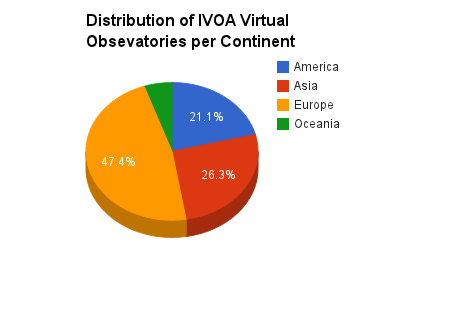
\includegraphics[width=0.5\textwidth]{img/ivoa_vos_distribution.png}
        %\caption{Distribución por continente de IVOA.}
    \end{center}
\end{figure}

Casi la mitad de los observatorios virtuales de IVOA están en Europa: 9 del
total; 1 pertenece a Oceanía, 4 a América y 5 de ellos a Asia \footnote{Como la
mayor parte de Rusia está en territorio Asiático, es considerado como uno de
los VO's de ese contintente.} 
\end{multicols}
\end{frame}

\newpage

\begin{frame}
\frametitle{Distribución si Chile es aceptado}
Si Chile se convirtiera en miembro de IVOA, la distribución sería la siguiente:
\newline

\begin{multicols}{2}
\begin{figure}[h!t]
    \begin{center}
       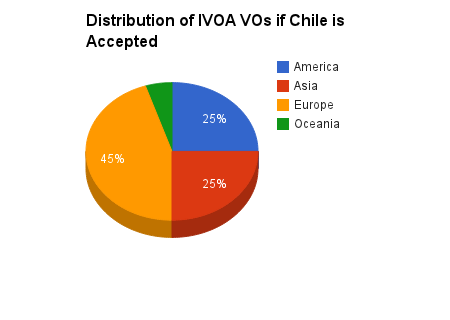
\includegraphics[width=0.5\textwidth]{img/if_chile_is_accepted.png}
       %\caption{International Virtual Observatory Alliance Distribución por continente incluyendo a Chile.}
    \end{center}
\end{figure}

La membresía de Chile igualaría la cantidad de VO's de Asia.  Este hecho
sería muy significativo, ya que un gran número de centros astronómicos como
observatorios están instalados en este país. Por ahora, se pretende trabajar
con datos del proyecto ALMA.
\end{multicols}

\end{frame}
